\documentclass[a4paper]{article}

\usepackage[utf8]{inputenc}
\usepackage[T1]{fontenc}
\usepackage[spanish]{babel}
\usepackage[margin={20mm,25mm}]{geometry}

\usepackage{ifthen}
\usepackage{mathtools}
\usepackage{xcolor}
\usepackage{booktabs}
\usepackage{circuitikz}
\usepackage{fancyhdr}
\usepackage{parskip}
\usepackage{hyperref}
\usepackage{graphicx}

% --------------------
% DATOS DEL INFORME
\newcommand{\numeroTarea}   {2}                 % <-- Reemplazar X con el número de la tarea
\newcommand{\numeroGrupo}   {22}                 % <-- Reemplazar N con el número de su grupo
\newcommand{\nombrePrimero} {Martín Arancibia Alvarado}    % <-- Reemplazar con el nombre del primer integrante
\newcommand{\rolPrimero}    {201973517-9}        % <-- Reemplazar con el rol del primer integrante
\newcommand{\nombreSegundo} {Miguel Soto Delgado}    % <-- Reemplazar con el nombre del segundo integrante
\newcommand{\rolSegundo}    {201973623-K}        % <-- Reemplazar con el rol del segundo integrante
% --------------------

% --------------------
% NO MODIFICAR ESTA PARTE
\title{Informe Tarea \numeroTarea \\ \large
    \ifthenelse{\equal{\numeroTarea}{1}}{Circuito Combinacional}{}
    \ifthenelse{\equal{\numeroTarea}{2}}{Circuito Secuencial}{}
    \ifthenelse{\equal{\numeroTarea}{3}}{Lenguajes de Descripción de Hardware}{}
    \ifthenelse{\equal{\numeroTarea}{4}}{ARM Assembly}{}
    \ifthenelse{\equal{\numeroTarea}{X}}{Tema de la tarea}{}
}
\author{\textbf{Grupo \numeroGrupo} \\ \begin{tabular}{r @{\quad} l}
    \nombrePrimero & \rolPrimero \\
    \nombreSegundo & \rolSegundo
\end{tabular}}
\date{\today}

\setlength{\parindent}{15pt}
\addto\captionsspanish{\renewcommand{\tablename}{Tabla}}
% --------------------

\begin{document}

\begin{titlepage}
    
    \vfill
    
    \begin{figure}
        
\includegraphics[width=0.3\textwidth]{logo_usm.png} % Con esto pueden incluir imágenes que hayan subido a Overleaf
    \end{figure}

    \maketitle
    % \thispagestyle{empty}
    
    \newpage

    \vfill
    \tableofcontents
\end{titlepage}

\newpage

\section{Resumen}

A lo largo de esta tarea se evaluarán los circuitos secuenciales, para ello, con la tarea previa que se hizo de circuitos combinacionales, se le aplicarán una serie de Latches y Flip Flops con el objetivo que el Exabot que se creó previamente pueda tener una cantidad de batería, gastarla y ser recargado con las distintas estaciones de carga. Junto a esto, también cumple con los distintos objetivos previamente dados en cuanto a las funciones de movimiento, revisando el estado actual de carga a la hora de tomar las decisiones de como moverse. Finalmente, las estaciones de carga ahora modifican el estado actual de la batería, devolviendo esta a 15 en caso de que el bot pase por una de ellas.



\newpage

\section{La batería}

La batería que se diseñará para esta tarea es la continuación de la tarea anterior, lo que cambia ahora es que debemos buscar que el nivel actual de la batería se determine en base a las condiciones en las que se encuentre en bot. En específico, los requerimientos son los siguientes:

\begin{itemize}
    \item La batería debe ser capáz de ser reiniciada a 15 una vez que tome una carga.
    \item La batería debe decrecer en 1 cada vez que se mueva y no haya una carga.
    \item La batería solo puede tomar un valor entero entre 0 y 15.
\end{itemize}

Este será el principal problema a resolver durante la tarea, y en la cuál nos enfocaremos de aquí en adante.

\newpage

\section{Estados de Carga}

En base a lo aprendido en clase, veremos que para solucionar el problema en cuestión, tendremos que hacer uso de los diferentes tipos de modelos
lógicos vistos. El nivel de carga puede verse como una máquina de estados finitos, en donde para cierto estado N, habrá un estado N+1 que le
procede. Visto en términos de la carga de forma concreta, tendremos los siguientes estados:

\\
\begin{center}
\begin{tabular}{ n | a | b | c | d } 
  \hline
	Número & $2^{0}$ & $2^{1}$ & $2^{2}$ & $2^{3}$ \\
  \hline
	0 & 0 & 0 & 0 & 0 \\
  \hline
	1 & 0 & 0 & 0 & 1 \\
  \hline
	2 & 0 & 0 & 1 & 0 \\
  \hline
	3 & 0 & 0 & 1 & 1 \\
  \hline
	4 & 0 & 1 & 0 & 0 \\
  \hline
	5 & 0 & 1 & 0 & 1 \\
  \hline
	6 & 0 & 1 & 1 & 0 \\
  \hline
	7 & 0 & 1 & 1 & 1 \\
  \hline
	8 & 1 & 0 & 0 & 0 \\
  \hline
	9 & 1 & 0 & 0 & 1 \\
  \hline
	10 & 1 & 0 & 1 & 0 \\
  \hline
	11 & 1 & 0 & 1 & 1 \\
  \hline
	12 & 1 & 1 & 0 & 0 \\
  \hline
	13 & 1 & 1 & 0 & 1 \\
  \hline
	14 & 1 & 1 & 1 & 0 \\
  \hline
	15 & 1 & 1 & 1 & 1 \\
\end{tabular}
\end{center}

Los cuáles serán obtenidos en orden decreciente, al ser parte de una batería que se consume por movimiento. Sumado a esto, tendremos que crear un
circuito que sea capáz de almacenar el estado actual de la batería para poder tomarlo como un input. Para esto será necesario el uso de registros.

\newpage

\section{Latches, Flip-Flops y Registros}

En vista de que para crear nuestro circuito no podemos utilizar Flip-Flops, ni latches ni Registros previamente definidos, tendremos que crear
los nuestros usando el Software Logisim, proceso que será detallado a continuación:

\subsection*{Latches}

Los latches serán parte crucial de nuestro modelo, ya que nos permitirán generar todo lo que viene a continuación. El tipo de Latch que usaremos
en específico es el SR Latch, el cuál nos permite definir un estado de entrada y reiniciarlo a conveniencia. Nuestro modelo del SR Latch quedó descrito de la siguiente manera en el software:

\begin{center}
	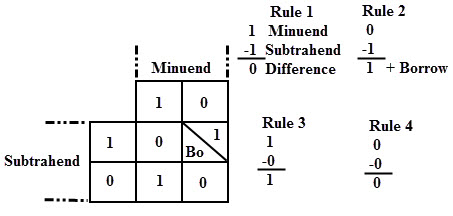
\includegraphics[width=0.4\textwidth]{tarea-2-ej-1.jpg}
\end{center}

Es importante recalcar que el estado se muestra como error, ya que el estado de un Latch se define por su entrada previa, como el Latch del esquema
no ha sido manipulado, su estado inicial está indefinido.

Posterior a esto, creamos un D Latch. Éste es contruído a partir del anterior, sin embargo este opera a través de la entrada de un reloj, el cuál permite
la actualización contínua de datos. Nuevamente, lo modelamos de la siguiente forma:

\begin{center}
	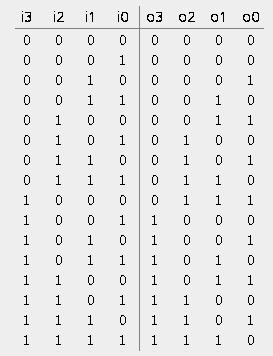
\includegraphics[width=0.55\textwidth]{tarea-2-ej-2.jpg}
\end{center}

\subsection*{Flip-Flops}

Los Latches descritos ahora nos servirán para crear lo que se llama un D Flip Flop, este nos permitirá finalmente almacenar un bit de forma contínua
en un sistema con reloj. Obtenido de la siguiente manera:

\begin{center}
	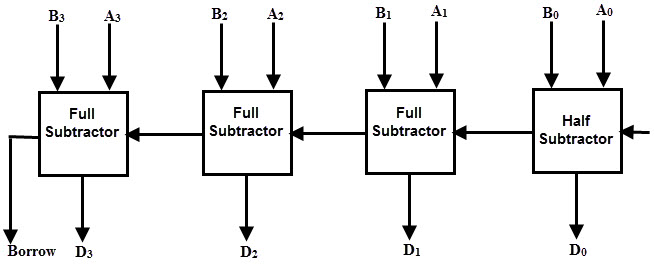
\includegraphics[width=0.7\textwidth]{tarea-2-ej-3.jpg}
\end{center}

Los D Flip Flops están construídos a partír de dos D Latches en una configuración llava "Maestro y Esclavo".

\subsection*{Registros}

Finalmente, poniéndo en uso todas las configuraciones mencionadas anteriormente, tendremos un registro. Para lo que nos compete en esta tarea, un
registro será un arreglo de N Flip Flops de tipo D, los cuáles nos permitirán almacenar N bits de memoria de forma simultánea. Para este ejercicio
en particular, nos permitirá almacenar los dígitos del valor de la batería para así poder disminuírlo con cada paso que el bot realize. El registro
que hicimos no será mostrado en esta sección ya que corresponde a lo que viene a continuación.

\newpage

\section{Contador}

El contador será el sistema final que nos permitirá saber el estado de la batería después de cierta cantidad de tiempo. Este contador consta de
un registro de 4 bits, el cuál conecta cada entrada con su propia salida para poder realizar un cheque contínuo del sistema, es decir, por cada
unidad de tiempo que pase, esta reducirá la cantidad de la batería (a menos de ser reiniciada en el caso de que el bot obtuviese una carga extra).
El esquema obtenido fue el siguiente:

\begin{center}
	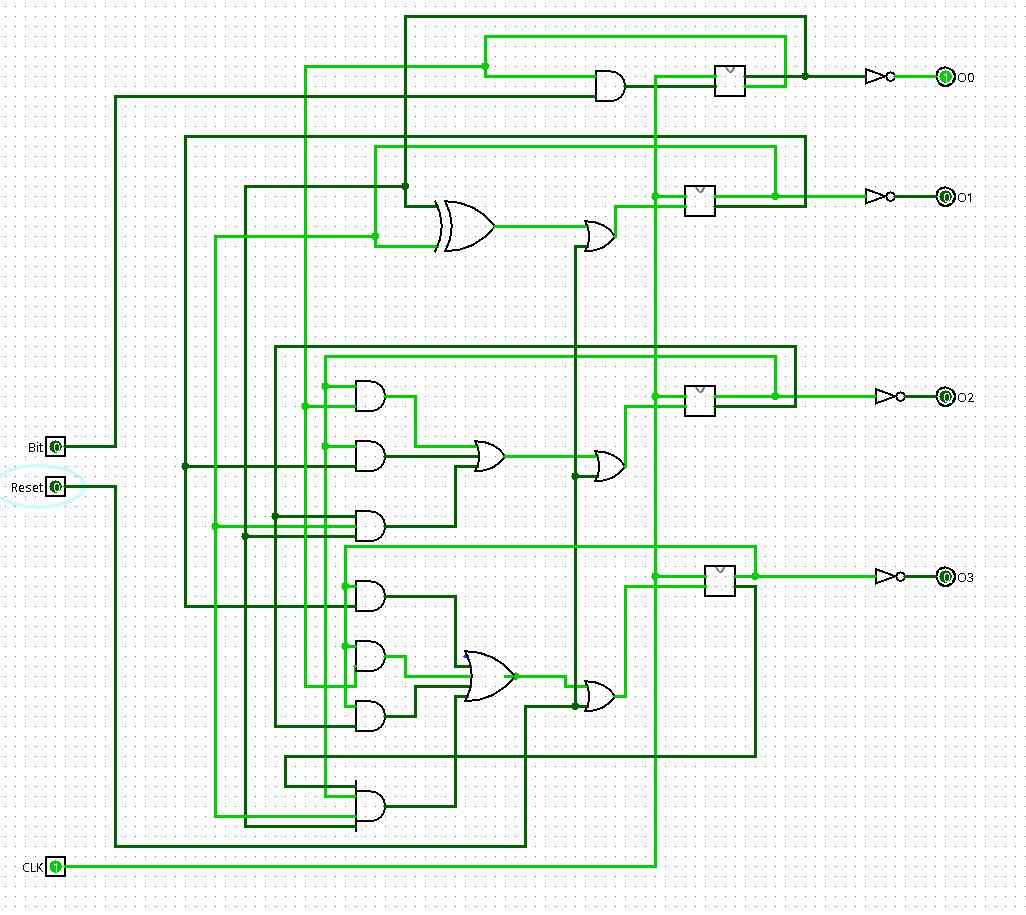
\includegraphics[width=0.8\textwidth]{tarea-2-ej-6.jpg}
\end{center}

La salida del sistema está representada por $O_{3}$, $O_{2}$, $O_{1}$ y $O_{0}$, cada uno de estos representando los dígitos del valor de la
batería. Hay un botón denominado "CLK" el cuál indica la entrada del reloj, en este caso es representado como un input normal ya que se pretende usar
dentro del sistema original descrito en la primera tarea. El contador posée un boton de "Reset" el cuál le permite reiniciar el sistema a 15 para 
cuando el bot recargue su batería. Y finalmente posée una entrada "Bit" el cuál sirve para indicar que el sistema está avanzando de forma normal.

\newpage

\section{Uniéndo Todo}

Finalmente, insertamos el nuevo circuíto en el sistema diseñado para la primera tarea, quedándonos de la siguiente manera:

\begin{center}
	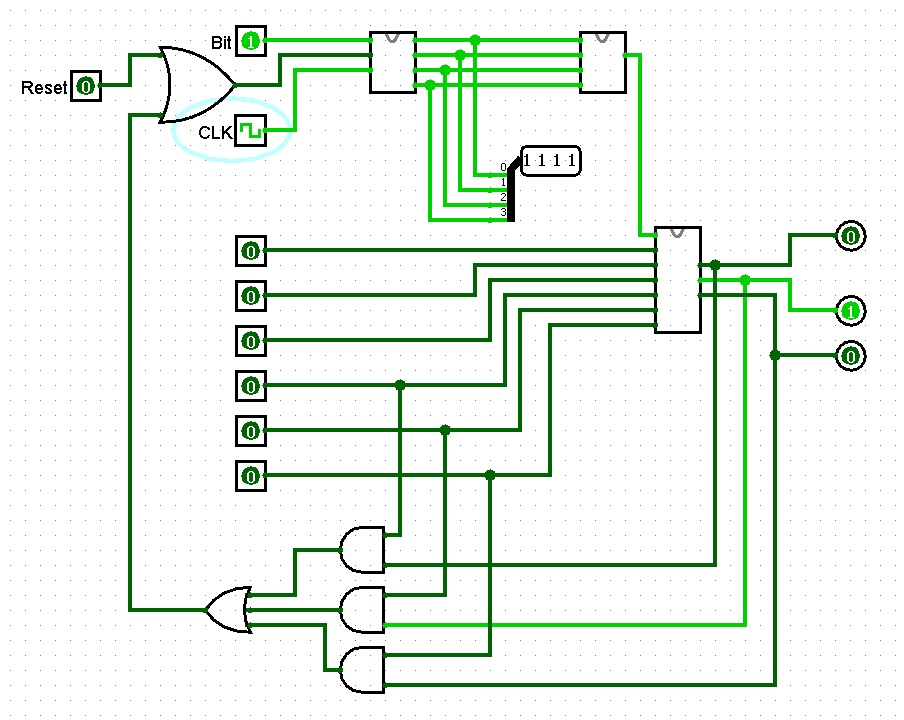
\includegraphics[width=0.8\textwidth]{tarea-2-ej-7.jpg}
\end{center}

El único inconveniente mayor es que el proceso de reinicio resulta un poco engorroso, consistiendo de los siguientes pasos a continuación:

1- Si recién se está activando por primera vez el circuito.

\begin{itemize}
	\item Dado cualquier estado, desactivar la entrada "Bit".
	\item Seguido de esto, activar el "Reset".
	\item Activar el reloj, dejando la batería en estado "0001".
	\item Desactivar el reloj y activar el "Bit", dejándo la batería en "0000".
	\item Avanzar el reloj un paso, dejándolo en el estado "1111" (el deseado).
\end{itemize}

2- En caso de resetearse por una estación de carga.

\begin{itemize}
	\item Activar el reloj, dejando la batería en estado "0000".
	\item Desactivar todos los inputs de entrada, dejando todos estos en "000000".
	\item Avanzar el reloj un paso, dejándolo en el estado "1111" (el deseado).
\end{itemize}


\newpage

\section{Resultado y análisis}

Para corroborar la efectividad de nuestro circuíto, lo sometimos a los casos de prueba entregados a través de Aula, dándonos las siguientes salidas:

\begin{center}
	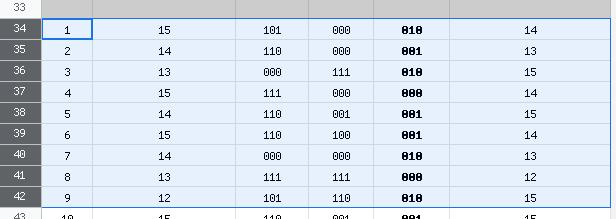
\includegraphics[width=0.8\textwidth]{tarea-2-casos.jpg}
\end{center}

Nuestros resultados al insertar dichos inputs:

\begin{center}
	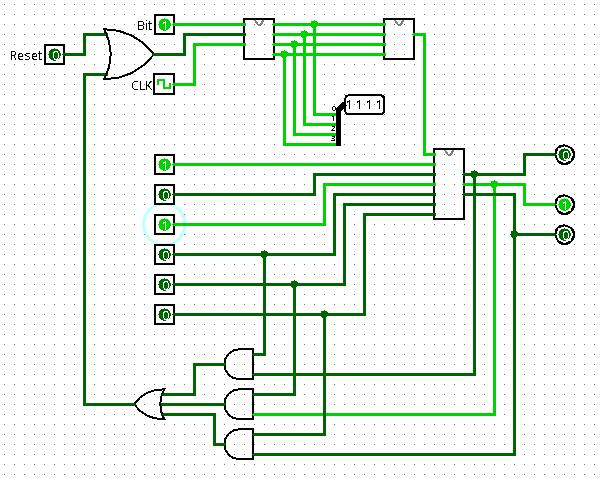
\includegraphics[width=0.6\textwidth]{tarea-2-prueba-34.jpg}
	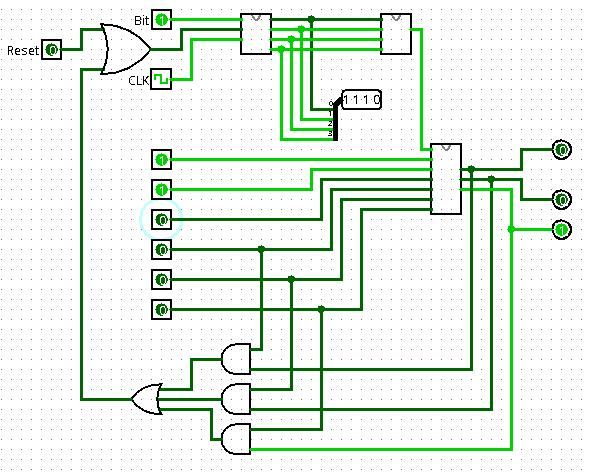
\includegraphics[width=0.6\textwidth]{tarea-2-prueba-35.jpg}
	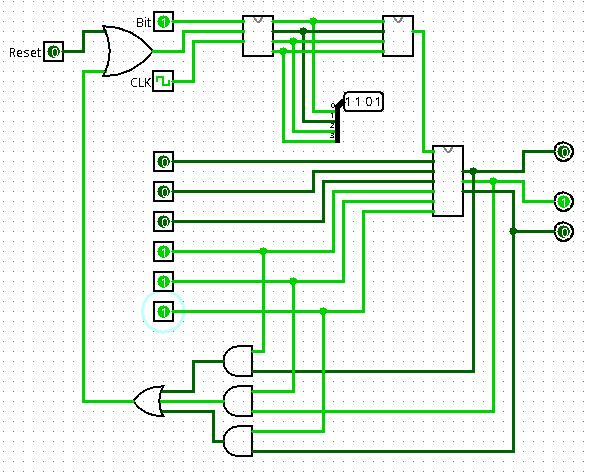
\includegraphics[width=0.6\textwidth]{tarea-2-prueba-36.jpg}
	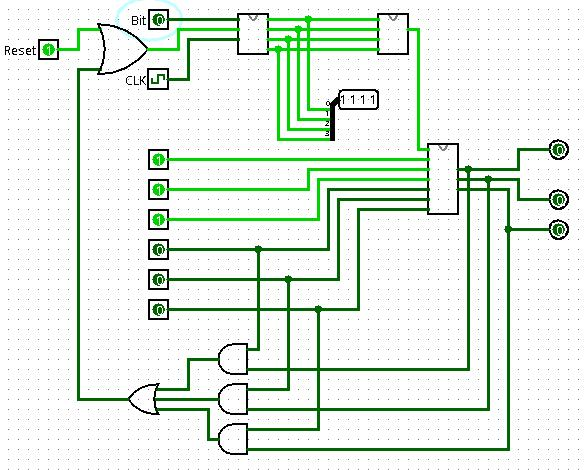
\includegraphics[width=0.6\textwidth]{tarea-2-prueba-37.jpg}
	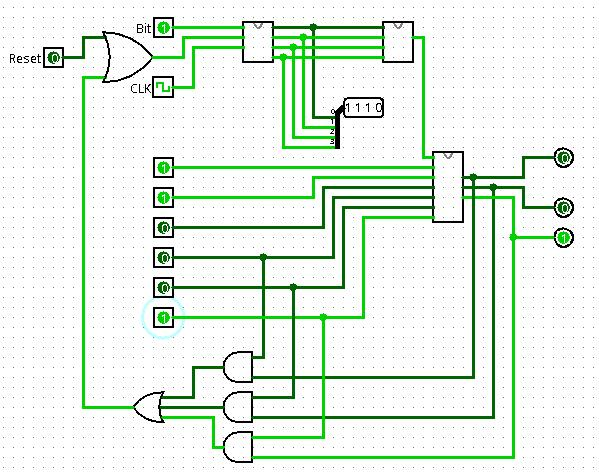
\includegraphics[width=0.6\textwidth]{tarea-2-prueba-38.jpg}
	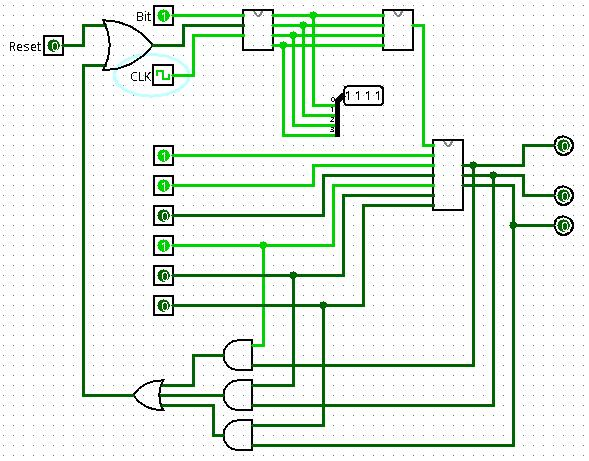
\includegraphics[width=0.6\textwidth]{tarea-2-prueba-39.jpg}
	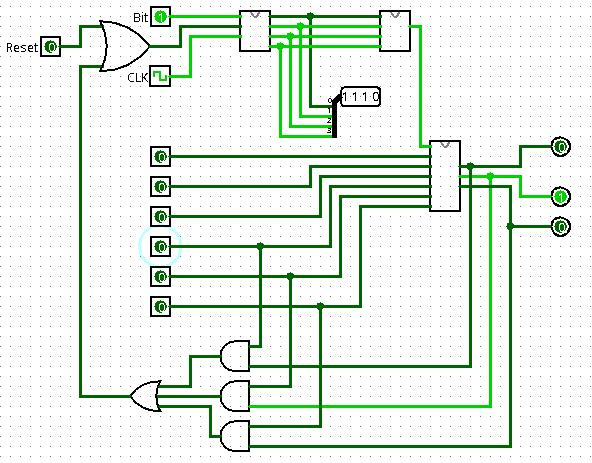
\includegraphics[width=0.6\textwidth]{tarea-2-prueba-40.jpg}
	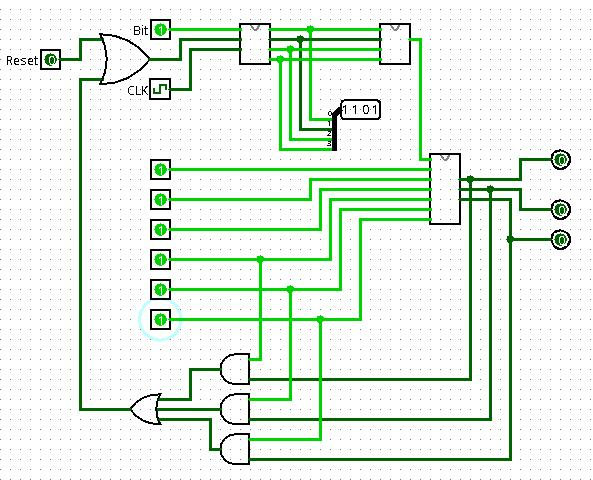
\includegraphics[width=0.6\textwidth]{tarea-2-prueba-41.jpg}
	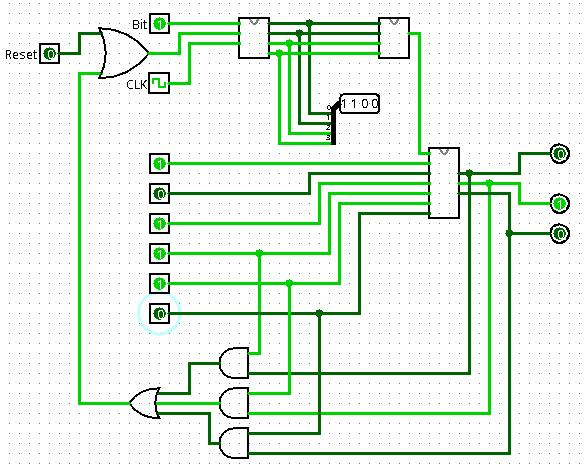
\includegraphics[width=0.6\textwidth]{tarea-2-prueba-42.jpg}
\end{center}

Podemos notar que de los casos de prueba, solo el paso 39 difiere del output presentado como pauta, por ende, nuestro circuito presenta ciertos errores. Más allá de eso, los resultados en los otros pasos son idénticos. Al indagar más al respecto, notamos que había un error de arrastre dentro de la tabla del movimiento del bot, esto fue arreglado posterior a la redacción del informe y por ende los resultados debiesen ser idénticos.

\newpage

\section{Conclusión}

La tarea nos presentó una gran necesidad del manejo correcto de los contenidos a lo largo de toda esta, ya que mientras desarrollabamos todo el material en varias ocasiones nos encontramos contra una pared grande, el cómo lograr lo que necesitabamos. Todo esto fue una lucha que tuvimos que hacer desde 0 al tener que crear nuestras propias herramientas de memoria y de contadores.

Con todas esas dificultades, sin embargo, se logró un aprendizaje alto y un gran despliegue de conocimientos que nos servirán a lo largo del curso, dominando contenidos a un nivel superior del previamente obtenido. Todo esto nos hace creer que como grupo logramos el objetivo de la tarea de aprender sobre los circuitos secuenciales y sus aplicaciones.

\newpage

\end{document}
